\chapter{Structural Patterns in Pin-wise MGXS}
\label{chap:spatial}

first paragraph: 
-

second paragraph:
-

%%%%%%%%%%%%%%%%%%%%%%%%%%%%%%%%%%%%%%%%%%%%%%%%%%%%%%%%%%%%%%%%%%%%%%%%%%%%%%%
\section{MGXS Clustering}


\begin{figure}[h!]
\centering
\begin{subfigure}{0.5\textwidth}
  \centering
  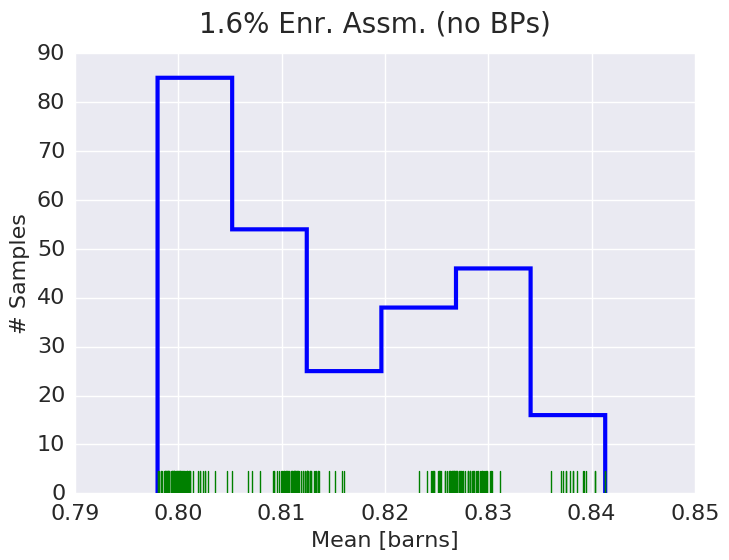
\includegraphics[width=\linewidth]{figures/patterns/assm-1.6/hist-kde-rug/assm-16-capt-1}
  \caption{}
  \label{fig:chap9-hist-assm-1.6-capt}
\end{subfigure}%
\begin{subfigure}{0.5\textwidth}
  \centering
  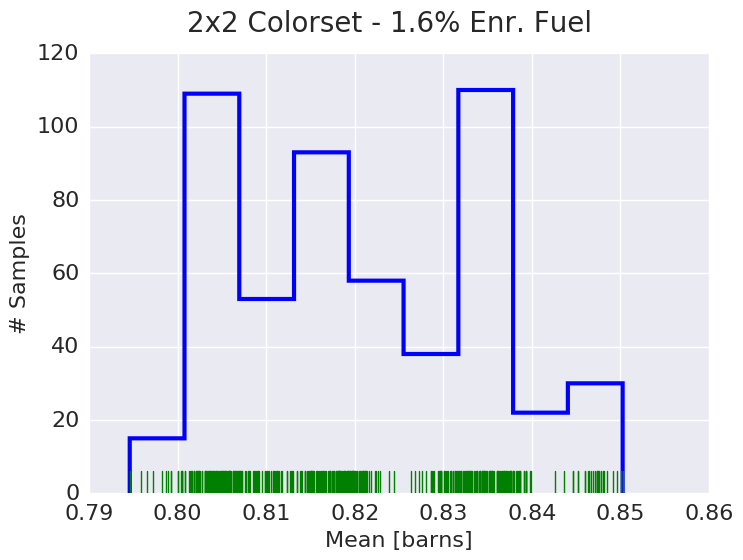
\includegraphics[width=\linewidth]{figures/patterns/2x2/hist-kde-rug/16-enr-capt-1}
  \caption{}
  \label{fig:chap9-hist-2x2-1.6-capt}
\end{subfigure}
\begin{subfigure}{0.5\textwidth}
  \centering
  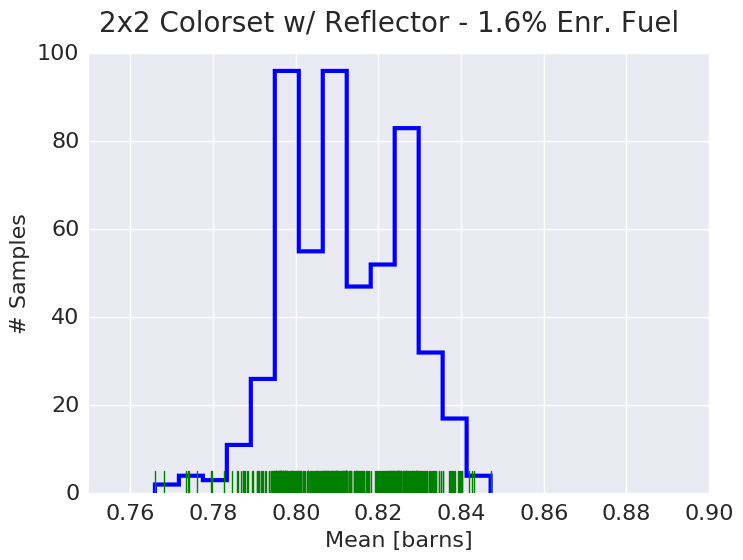
\includegraphics[width=\linewidth]{figures/patterns/reflector/hist-kde-rug/16-enr-capt-1}  \caption{}
  \label{fig:chap9-hist-reflector-1.6-capt}
\end{subfigure}%
\begin{subfigure}{0.5\textwidth}
  \centering
  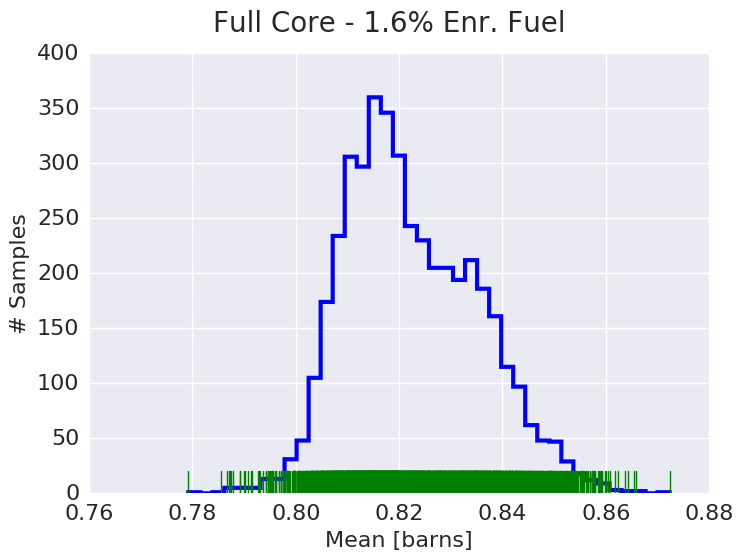
\includegraphics[width=\linewidth]{figures/patterns/full-core/hist-kde-rug/16-enr-capt-1} \caption{}
  \label{fig:chap9-hist-full-core-1.6-capt}
\end{subfigure}
\caption[Histogram of U-238 capture MGXS for 1.6\% enriched fuel]{Histograms of U-238 capture \ac{MGXS} for 1.6\% enriched fuel.}
\label{fig:chap9-hist-1.6-capt}
\end{figure}

\begin{figure}[h!]
\centering
\begin{subfigure}{0.5\textwidth}
  \centering
  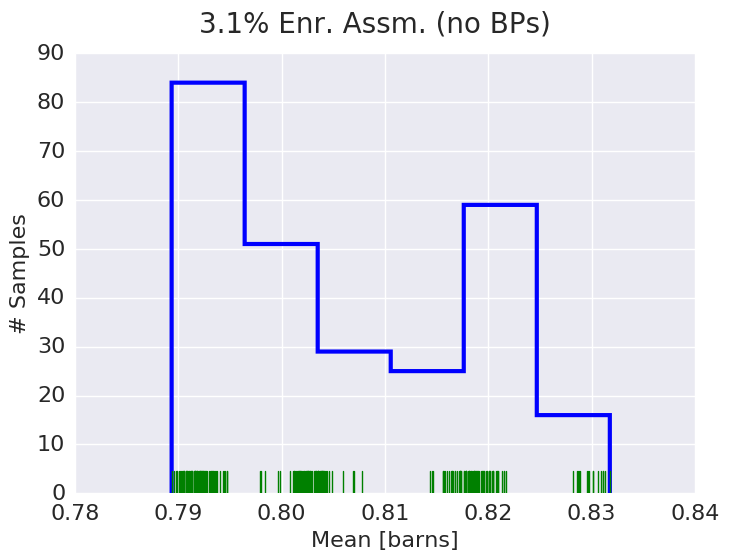
\includegraphics[width=\linewidth]{figures/patterns/assm-3.1/hist-kde-rug/assm-31-capt-1}
  \caption{}
  \label{fig:chap9-hist-assm-3.1-capt}
\end{subfigure}%
\begin{subfigure}{0.5\textwidth}
  \centering
  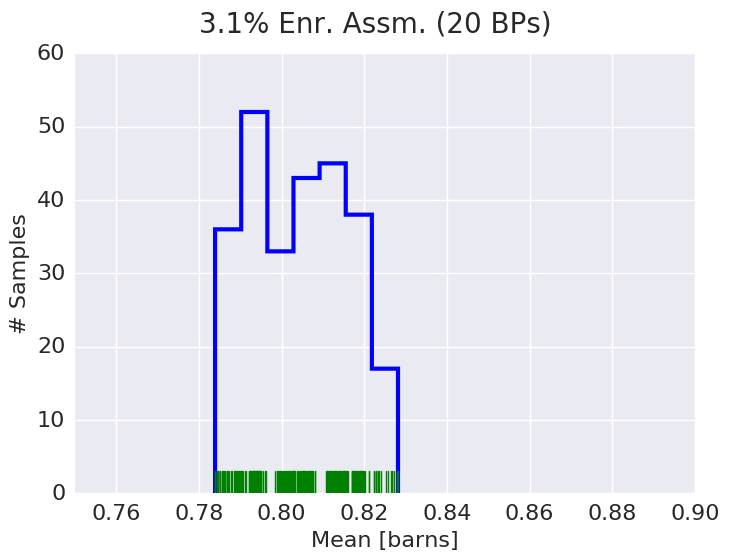
\includegraphics[width=\linewidth]{figures/patterns/assm-3.1-20BPs/hist-kde-rug/assm-31-20BPs-capt-1}
  \caption{}
  \label{fig:chap9-hist-assm-3.1-20BPs-capt}
\end{subfigure}
\begin{subfigure}{0.5\textwidth}
  \centering
  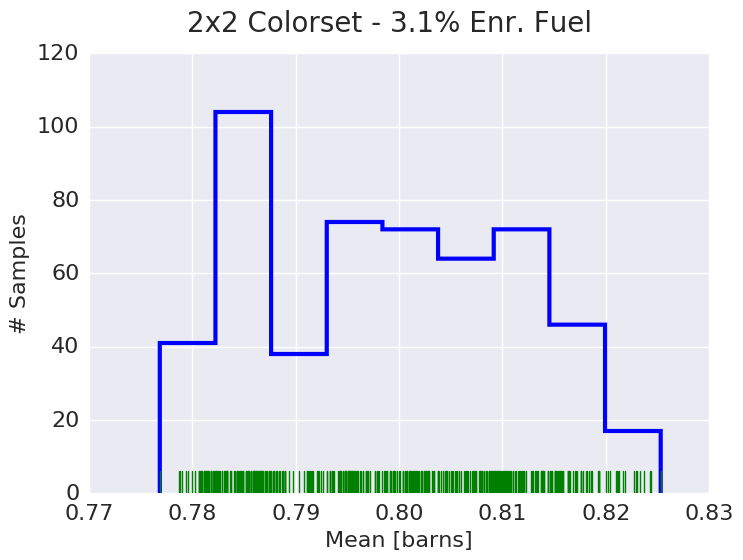
\includegraphics[width=\linewidth]{figures/patterns/2x2/hist-kde-rug/31-enr-capt-1}
  \caption{}
  \label{fig:chap9-hist-2x2-3.1-capt}
\end{subfigure}%
\begin{subfigure}{0.5\textwidth}
  \centering
  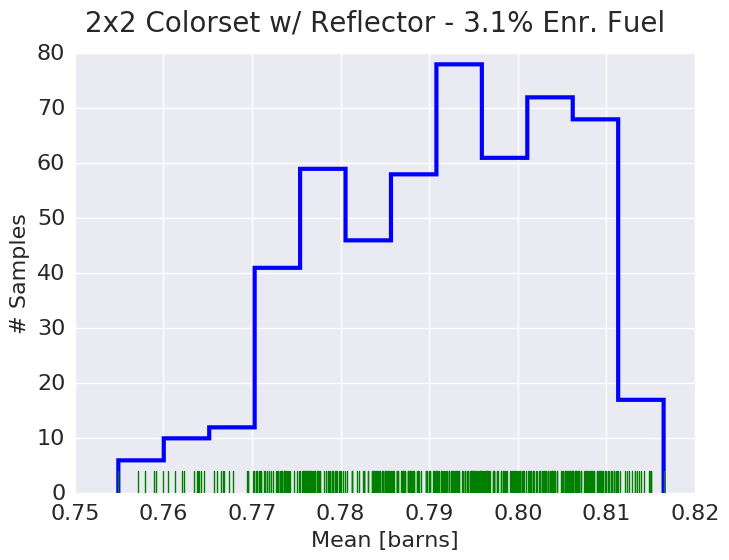
\includegraphics[width=\linewidth]{figures/patterns/reflector/hist-kde-rug/31-enr-capt-1}  \caption{}
  \label{fig:chap9-hist-reflector-3.1-capt}
\end{subfigure}
\begin{subfigure}{0.5\textwidth}
  \centering
  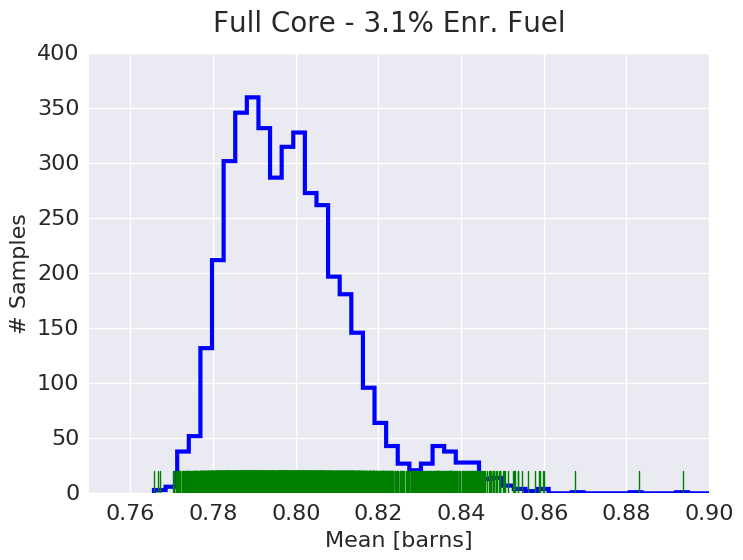
\includegraphics[width=\linewidth]{figures/patterns/full-core/hist-kde-rug/31-enr-capt-1} \caption{}
  \label{fig:chap9-hist-full-core-3.1-capt}
\end{subfigure}
\caption[Histogram of U-238 capture MGXS for 3.1\% enriched fuel]{Histograms of U-238 capture \ac{MGXS} for 3.1\% enriched fuel.}
\label{fig:chap9-hist-3.1-capt}
\end{figure}


\begin{figure}[h!]
\centering
\begin{subfigure}{0.5\textwidth}
  \centering
  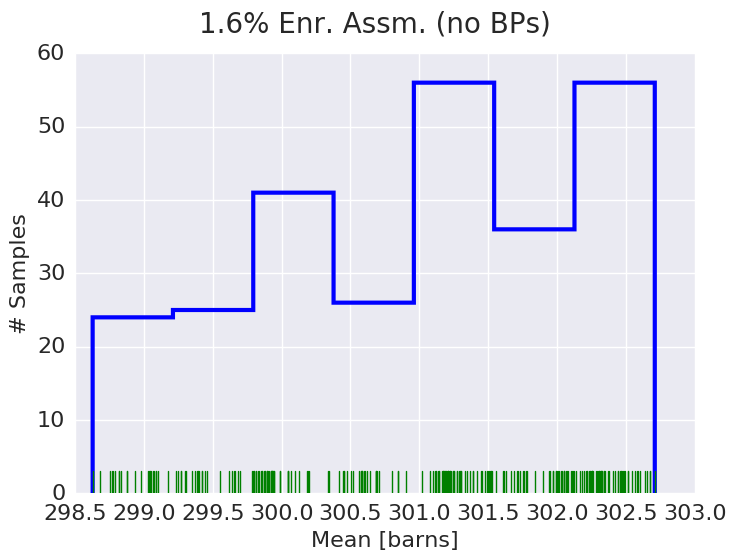
\includegraphics[width=\linewidth]{figures/patterns/assm-1.6/hist-kde-rug/assm-16-fiss-2}
  \caption{}
  \label{fig:chap9-hist-assm-1.6-fiss}
\end{subfigure}%
\begin{subfigure}{0.5\textwidth}
  \centering
  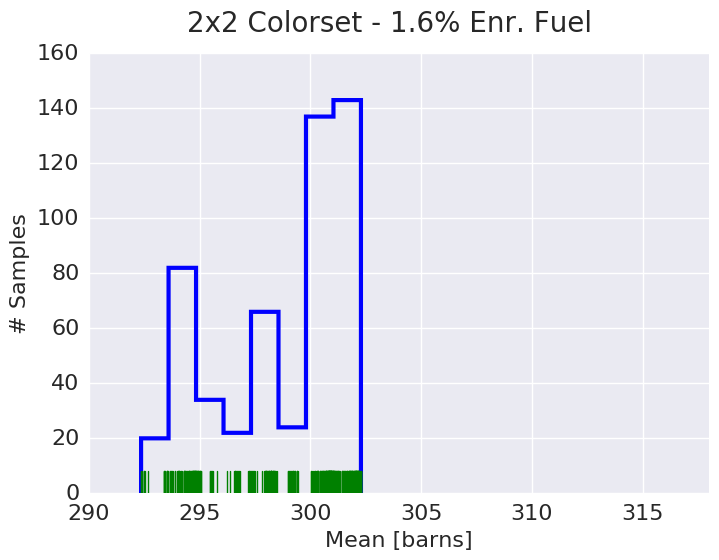
\includegraphics[width=\linewidth]{figures/patterns/2x2/hist-kde-rug/16-enr-fiss-2}
  \caption{}
  \label{fig:chap9-hist-2x2-1.6-fiss}
\end{subfigure}
\begin{subfigure}{0.5\textwidth}
  \centering
  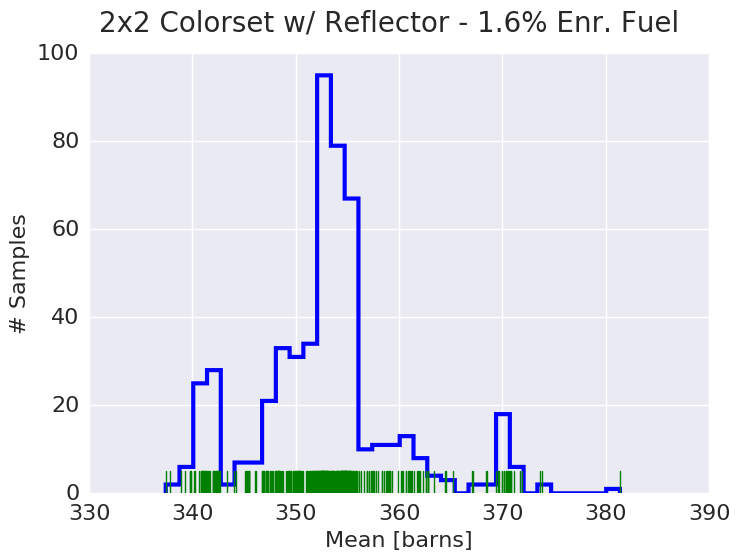
\includegraphics[width=\linewidth]{figures/patterns/reflector/hist-kde-rug/16-enr-fiss-2}  \caption{}
  \label{fig:chap9-hist-reflector-1.6-fiss}
\end{subfigure}%
\begin{subfigure}{0.5\textwidth}
  \centering
  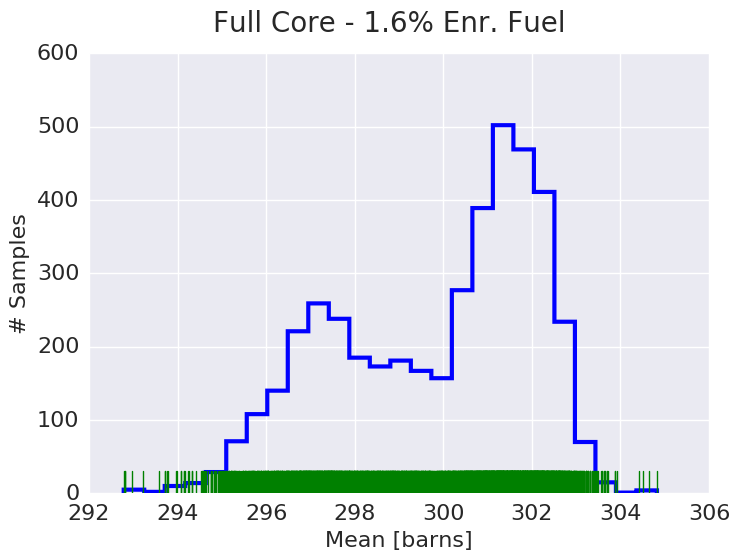
\includegraphics[width=\linewidth]{figures/patterns/full-core/hist-kde-rug/16-enr-fiss-2} \caption{}
  \label{fig:chap9-hist-full-core-1.6-fiss}
\end{subfigure}
\caption[Histogram of U-235 fission MGXS for 1.6\% enriched fuel]{Histograms of U-235 fission \ac{MGXS} for 1.6\% enriched fuel.}
\label{fig:chap9-hist-1.6-fiss}
\end{figure}

\begin{figure}[h!]
\centering
\begin{subfigure}{0.5\textwidth}
  \centering
  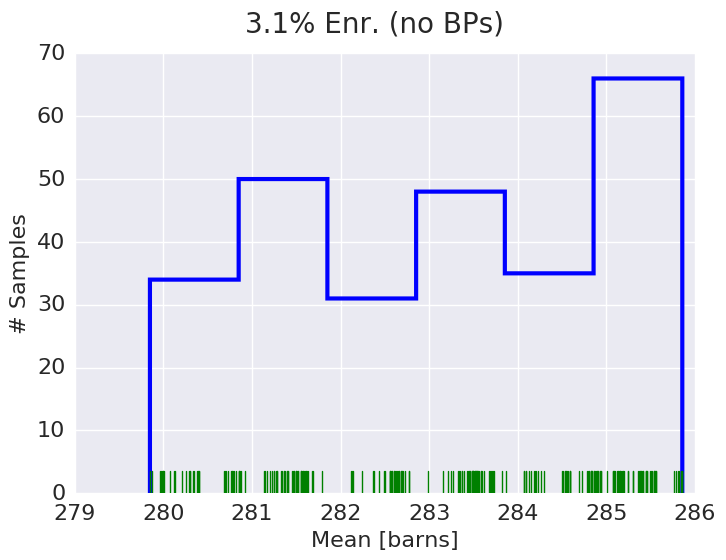
\includegraphics[width=\linewidth]{figures/patterns/assm-3.1/hist-kde-rug/assm-31-fiss-2}
  \caption{}
  \label{fig:chap9-hist-assm-3.1-fiss}
\end{subfigure}%
\begin{subfigure}{0.5\textwidth}
  \centering
  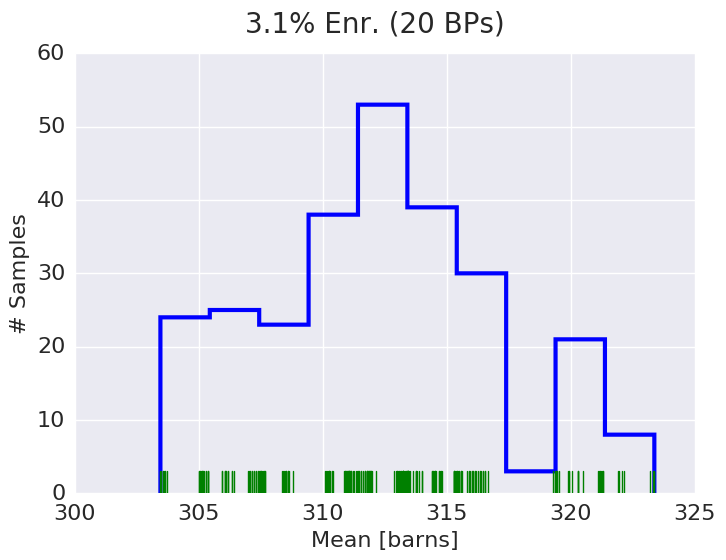
\includegraphics[width=\linewidth]{figures/patterns/assm-3.1-20BPs/hist-kde-rug/assm-31-20BPs-fiss-2}
  \caption{}
  \label{fig:chap9-hist-assm-3.1-20BPs-fiss}
\end{subfigure}
\begin{subfigure}{0.5\textwidth}
  \centering
  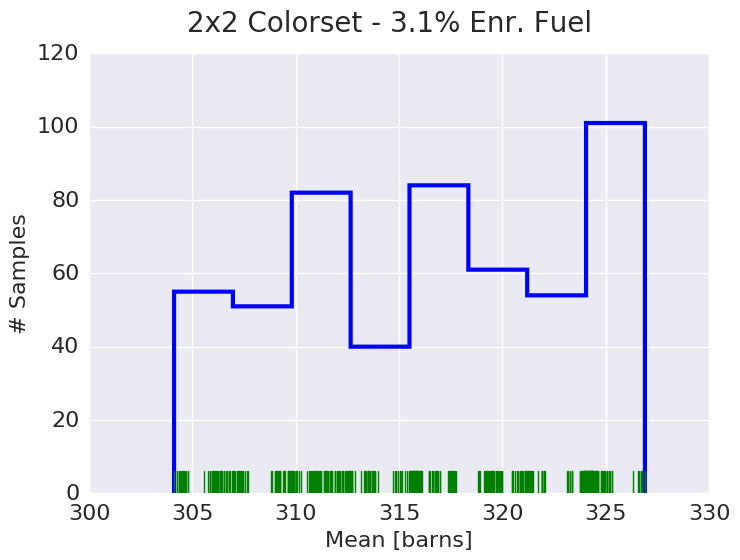
\includegraphics[width=\linewidth]{figures/patterns/2x2/hist-kde-rug/31-enr-fiss-2}
  \caption{}
  \label{fig:chap9-hist-2x2-3.1-fiss}
\end{subfigure}%
\begin{subfigure}{0.5\textwidth}
  \centering
  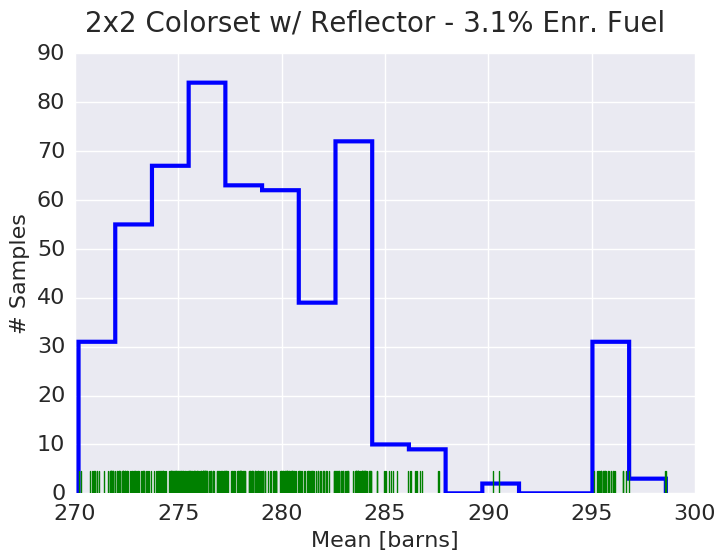
\includegraphics[width=\linewidth]{figures/patterns/reflector/hist-kde-rug/31-enr-fiss-2}  \caption{}
  \label{fig:chap9-hist-reflector-3.1-fiss}
\end{subfigure}
\begin{subfigure}{0.5\textwidth}
  \centering
  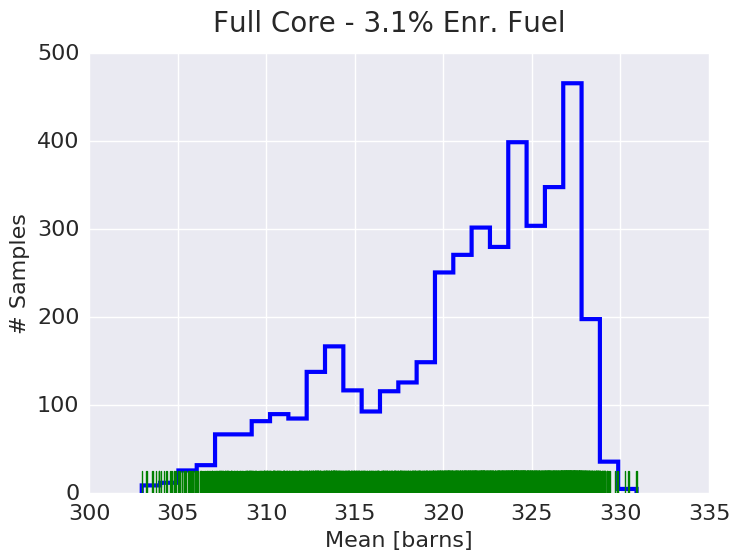
\includegraphics[width=\linewidth]{figures/patterns/full-core/hist-kde-rug/31-enr-fiss-2} \caption{}
  \label{fig:chap9-hist-full-core-3.1-fiss}
\end{subfigure}
\caption[Histogram of U-235 fission MGXS 3.1\% enriched fuel]{Histograms of U-235 fission \ac{MGXS} for 3.1\% enriched fuel.}
\label{fig:chap9-hist-3.1-fiss}
\end{figure}










\begin{figure}[h!]
\centering
\begin{subfigure}{0.5\textwidth}
  \centering
  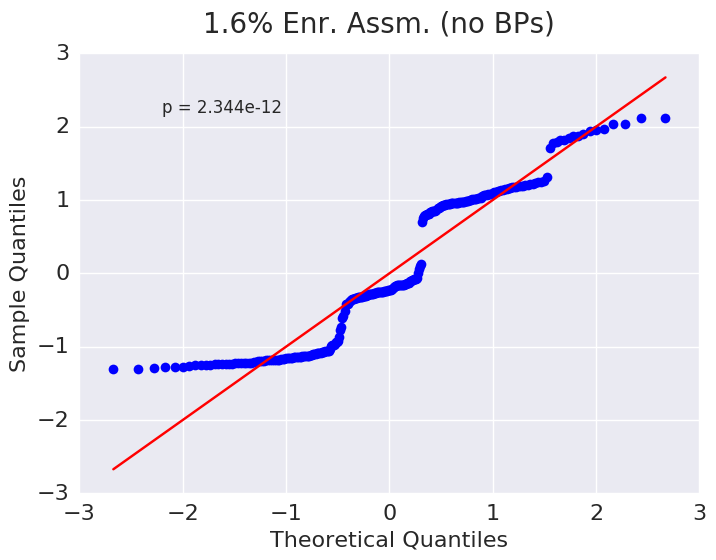
\includegraphics[width=\linewidth]{figures/patterns/assm-1.6/quantile/assm-16-capt-1}
  \caption{}
  \label{fig:chap9-qq-assm-1.6-capt}
\end{subfigure}%
\begin{subfigure}{0.5\textwidth}
  \centering
  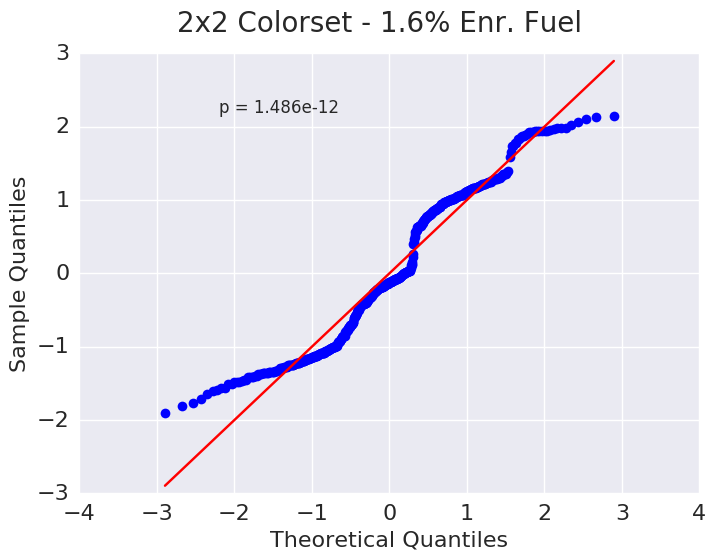
\includegraphics[width=\linewidth]{figures/patterns/2x2/quantile/16-enr-capt-1}
  \caption{}
  \label{fig:chap9-qq-2x2-1.6-capt}
\end{subfigure}
\begin{subfigure}{0.5\textwidth}
  \centering
  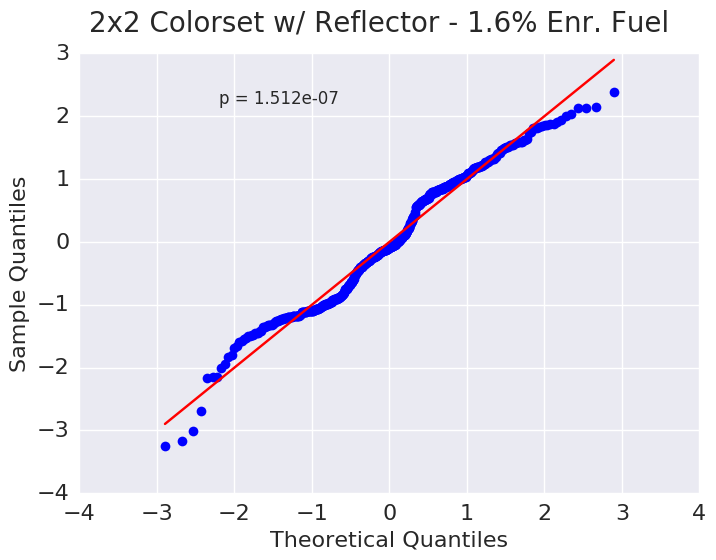
\includegraphics[width=\linewidth]{figures/patterns/reflector/quantile/16-enr-capt-1}  \caption{}
  \label{fig:chap9-qq-reflector-1.6-capt}
\end{subfigure}%
\begin{subfigure}{0.5\textwidth}
  \centering
  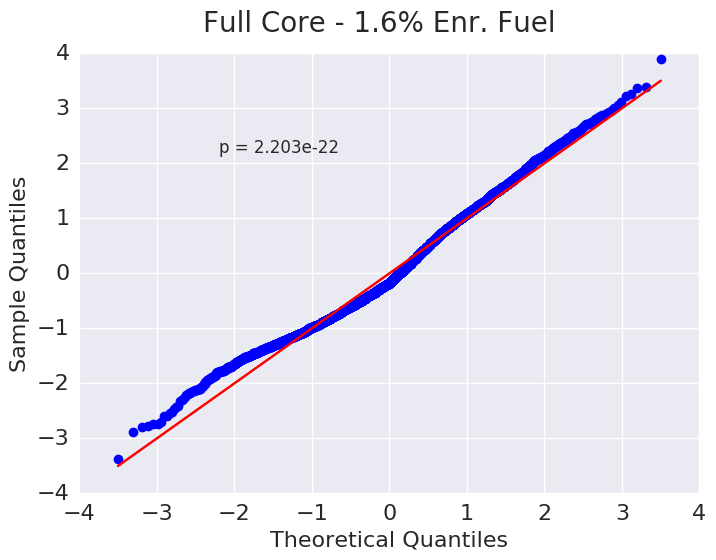
\includegraphics[width=\linewidth]{figures/patterns/full-core/quantile/16-enr-capt-1} \caption{}
  \label{fig:chap9-qq-full-core-1.6-capt}
\end{subfigure}
\caption[Q-Q plots of U-238 capture MGXS for 1.6\% enriched fuel]{Q-Q plots of U-238 capture \ac{MGXS} for 1.6\% enriched fuel.}
\label{fig:chap9-qq-1.6-capt}
\end{figure}

\begin{figure}[h!]
\centering
\begin{subfigure}{0.5\textwidth}
  \centering
  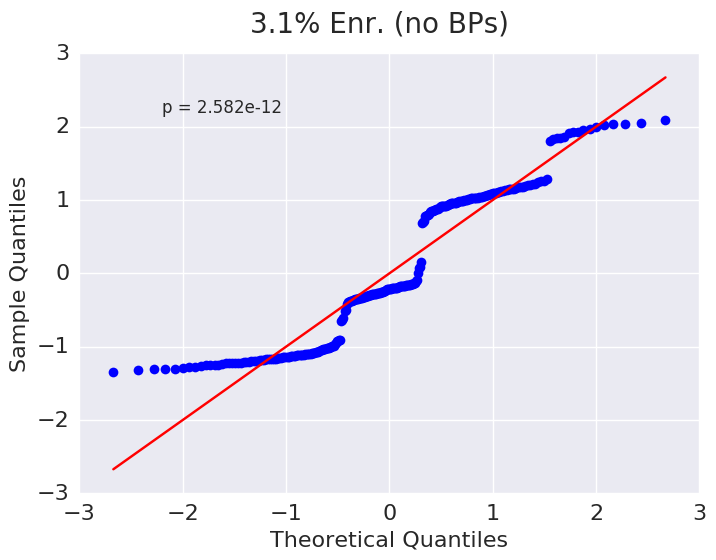
\includegraphics[width=\linewidth]{figures/patterns/assm-3.1/quantile/assm-31-capt-1}
  \caption{}
  \label{fig:chap9-qq-assm-3.1-capt}
\end{subfigure}%
\begin{subfigure}{0.5\textwidth}
  \centering
  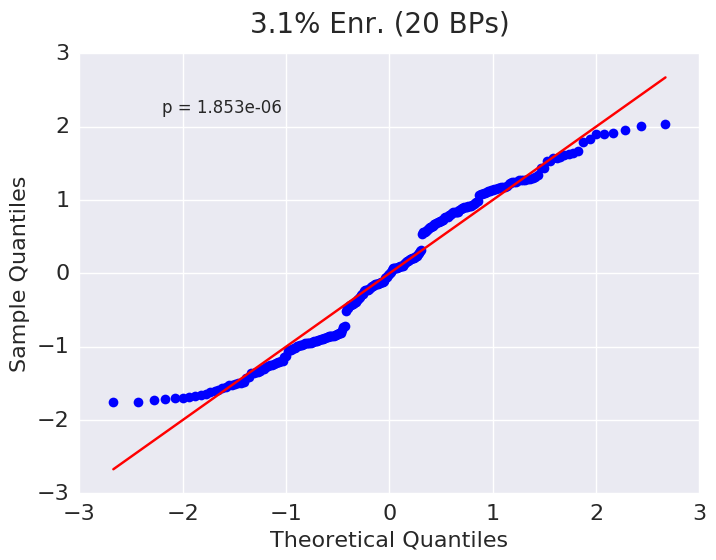
\includegraphics[width=\linewidth]{figures/patterns/assm-3.1-20BPs/quantile/assm-31-20BPs-capt-1}
  \caption{}
  \label{fig:chap9-qq-assm-3.1-20BPs-capt}
\end{subfigure}
\begin{subfigure}{0.5\textwidth}
  \centering
  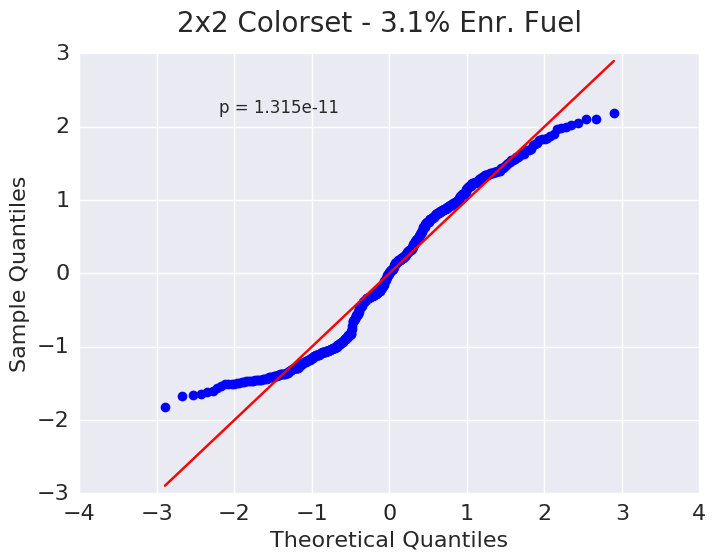
\includegraphics[width=\linewidth]{figures/patterns/2x2/quantile/31-enr-capt-1}
  \caption{}
  \label{fig:chap9-qq-2x2-3.1-capt}
\end{subfigure}%
\begin{subfigure}{0.5\textwidth}
  \centering
  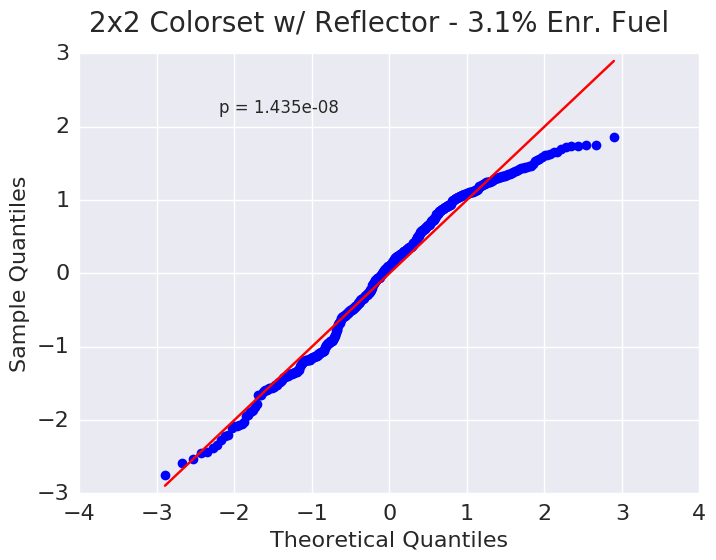
\includegraphics[width=\linewidth]{figures/patterns/reflector/quantile/31-enr-capt-1}  \caption{}
  \label{fig:chap9-qq-reflector-3.1-capt}
\end{subfigure}
\begin{subfigure}{0.5\textwidth}
  \centering
  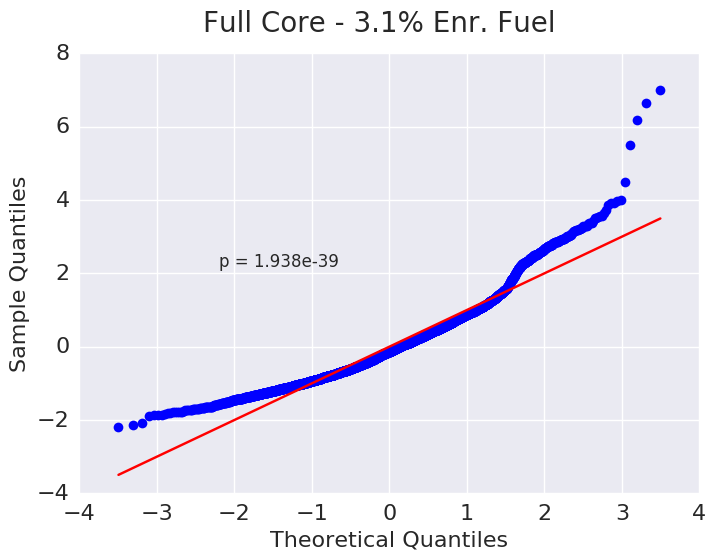
\includegraphics[width=\linewidth]{figures/patterns/full-core/quantile/31-enr-capt-1} \caption{}
  \label{fig:chap9-qq-full-core-3.1-capt}
\end{subfigure}
\caption[Q-Q plots of U-238 capture MGXS for 3.1\% enriched fuel]{Q-Q plots of U-238 capture \ac{MGXS} for 3.1\% enriched fuel.}
\label{fig:chap9-qq-3.1-capt}
\end{figure}


\begin{figure}[h!]
\centering
\begin{subfigure}{0.5\textwidth}
  \centering
  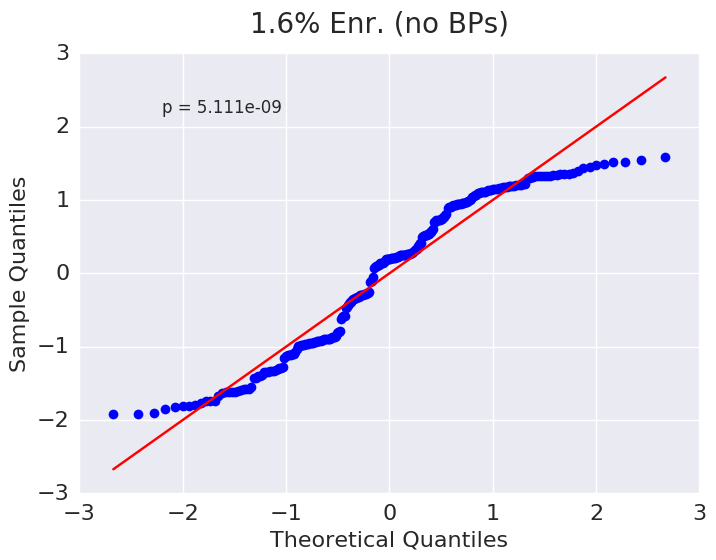
\includegraphics[width=\linewidth]{figures/patterns/assm-1.6/quantile/assm-16-fiss-2}
  \caption{}
  \label{fig:chap9-qq-assm-1.6-fiss}
\end{subfigure}%
\begin{subfigure}{0.5\textwidth}
  \centering
  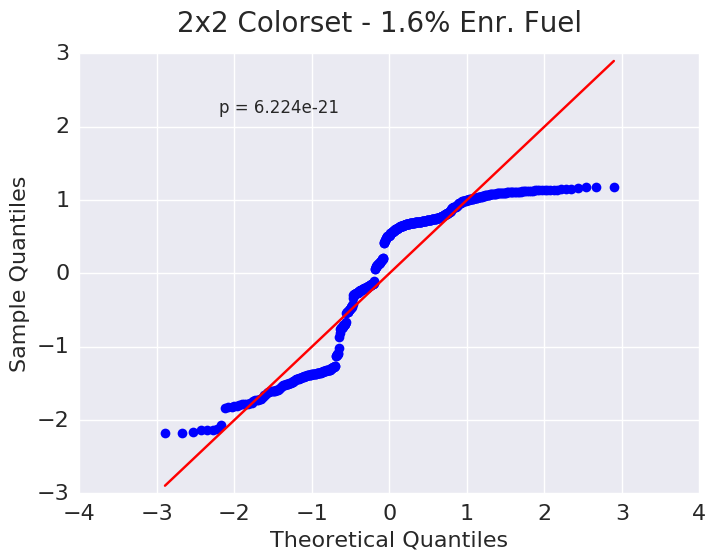
\includegraphics[width=\linewidth]{figures/patterns/2x2/quantile/16-enr-fiss-2}
  \caption{}
  \label{fig:chap9-qq-2x2-1.6-fiss}
\end{subfigure}
\begin{subfigure}{0.5\textwidth}
  \centering
  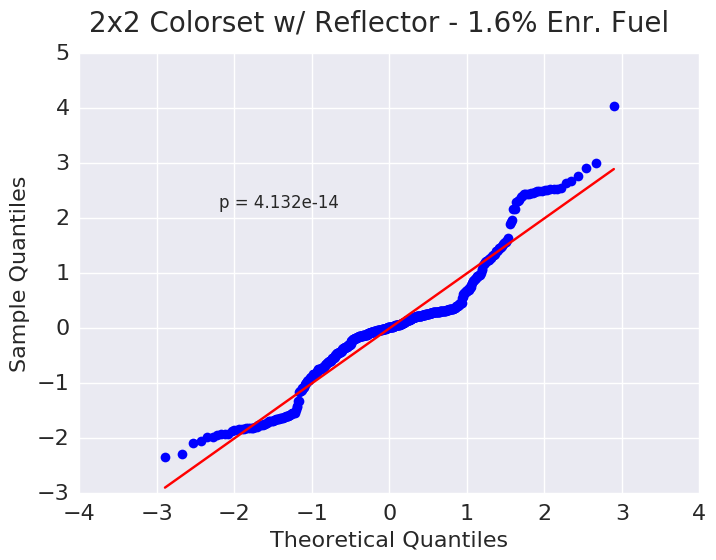
\includegraphics[width=\linewidth]{figures/patterns/reflector/quantile/16-enr-fiss-2}  \caption{}
  \label{fig:chap9-qq-reflector-1.6-fiss}
\end{subfigure}%
\begin{subfigure}{0.5\textwidth}
  \centering
  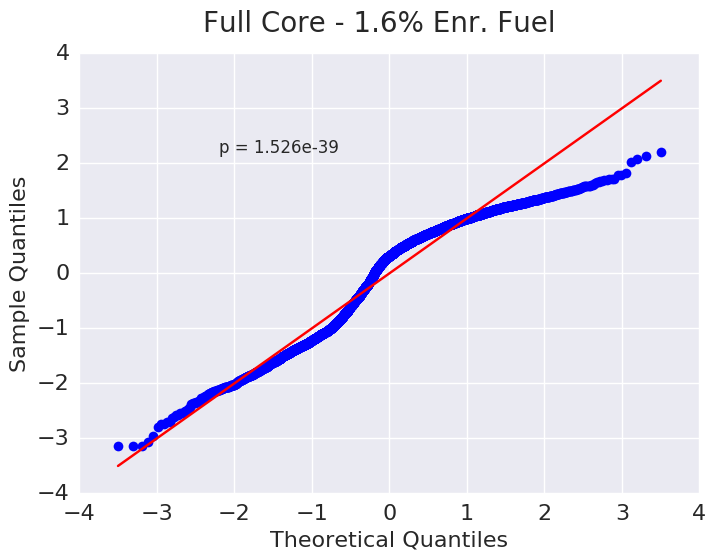
\includegraphics[width=\linewidth]{figures/patterns/full-core/quantile/16-enr-fiss-2} \caption{}
  \label{fig:chap9-qq-full-core-1.6-fiss}
\end{subfigure}
\caption[Q-Q plots of U-235 fission MGXS for 1.6\% enriched fuel]{Q-Q plots of U-235 fission \ac{MGXS} for 1.6\% enriched fuel.}
\label{fig:chap9-qq-1.6-fiss}
\end{figure}

\begin{figure}[h!]
\centering
\begin{subfigure}{0.5\textwidth}
  \centering
  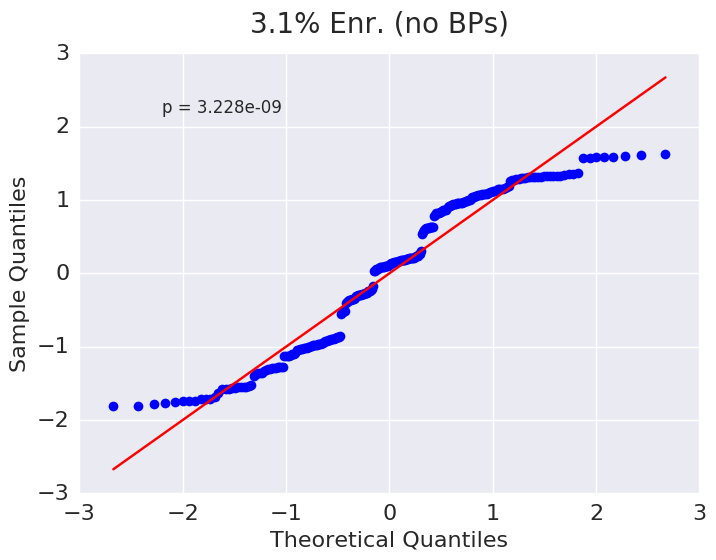
\includegraphics[width=\linewidth]{figures/patterns/assm-3.1/quantile/assm-31-fiss-2}
  \caption{}
  \label{fig:chap9-qq-assm-3.1-fiss}
\end{subfigure}%
\begin{subfigure}{0.5\textwidth}
  \centering
  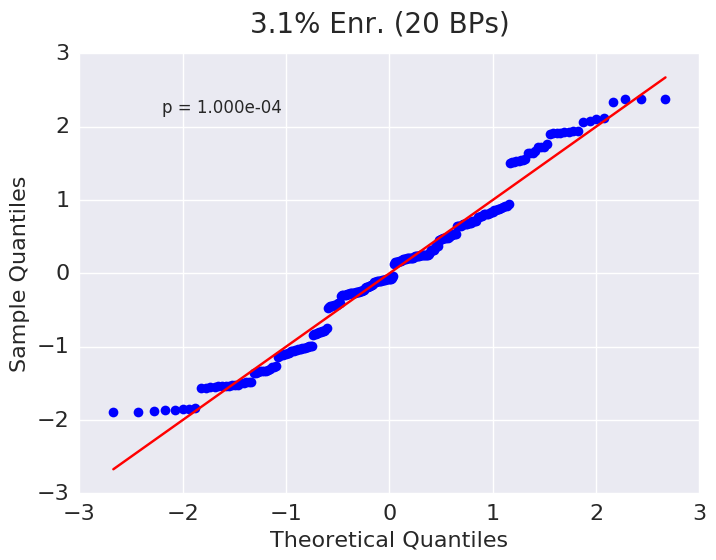
\includegraphics[width=\linewidth]{figures/patterns/assm-3.1-20BPs/quantile/assm-31-20BPs-fiss-2}
  \caption{}
  \label{fig:chap9-qq-assm-3.1-20BPs-fiss}
\end{subfigure}
\begin{subfigure}{0.5\textwidth}
  \centering
  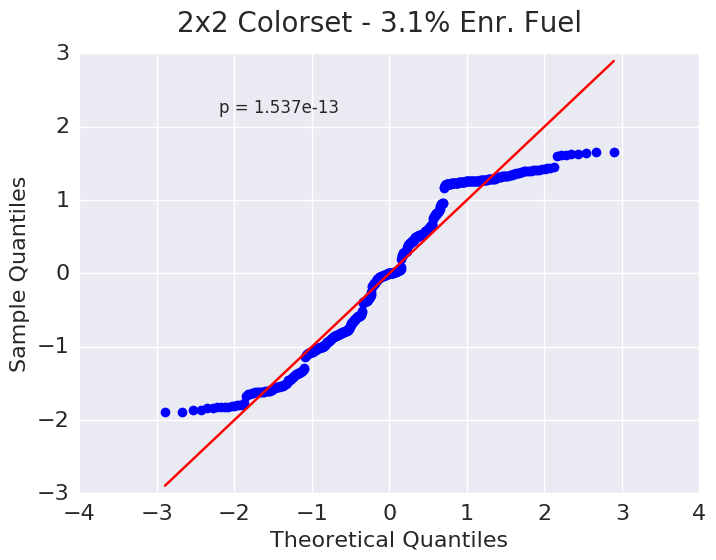
\includegraphics[width=\linewidth]{figures/patterns/2x2/quantile/31-enr-fiss-2}
  \caption{}
  \label{fig:chap9-qq-2x2-3.1-fiss}
\end{subfigure}%
\begin{subfigure}{0.5\textwidth}
  \centering
  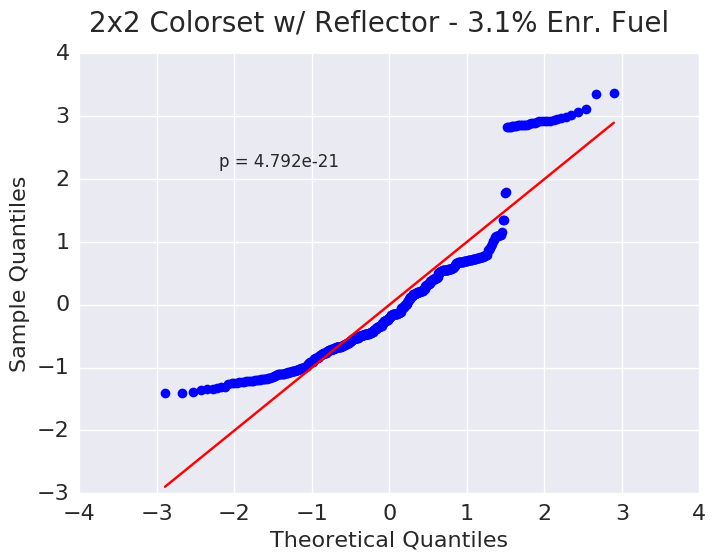
\includegraphics[width=\linewidth]{figures/patterns/reflector/quantile/31-enr-fiss-2}  \caption{}
  \label{fig:chap9-qq-reflector-3.1-fiss}
\end{subfigure}
\begin{subfigure}{0.5\textwidth}
  \centering
  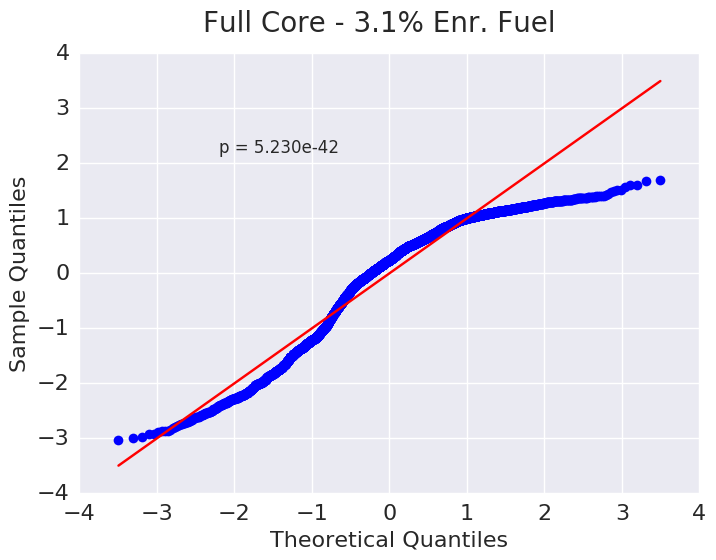
\includegraphics[width=\linewidth]{figures/patterns/full-core/quantile/31-enr-fiss-2} \caption{}
  \label{fig:chap9-qq-full-core-3.1-fiss}
\end{subfigure}
\caption[Q-Q plots of U-235 fission MGXS 3.1\% enriched fuel]{Q-Q plots of U-235 fission \ac{MGXS} for 3.1\% enriched fuel.}
\label{fig:chap9-qq-3.1-fiss}
\end{figure}




first paragraph:
-

second paragraph:
-

-want to look at all five benchmarks in succession with different MGXS clusters
  -plots of U-238 capture (group 27/1); U-235 fission (group 65/2)
    -octo plots
    -histrogram/rug/kde
    -QQ plots
-need to plot for both assemblies in colorsets
-need to plot for all three enrichments for BEAVRS
  
-look at slides 66-71 in ORNL presentation

\begin{itemize}[noitemsep]
  \item show that clustering exists in MGXS
  \begin{itemize}[noitemsep]
    \item leave ``features'' and ML discussion for next chapter
  \end{itemize}
  \item histogram / rug plots of clustered MGXS
  \item quantile-quantile plots  
\end{itemize}


%%%%%%%%%%%%%%%%%%%%%%%%%%%%%%%%%%%%%%%%%%%%%%%%%%%%%%%%%%%%%%%%%%%%%%%%%%%%%%%
\section{Pin-Wise Population Variance}

-plot the convergence of null MGXS by batch along with max for distribcell MGXS
-plot the pop. var. convergence of the distribcell MGXS and show that they don't go to zero
-plot the convergence of the distribcell MGXS for 1.6\% enr. assm, 3.1\% assm w/ BPs, 2x2 colorset w/ reflector???

\begin{itemize}[noitemsep]
  \item table of population variance of distribcell MGXS
  \item plots of convergence of pop. var. of distribell MGXS
  \begin{itemize}[noitemsep]
    \item MGXS in moderator and fuel
    \item pop. var. in fuel converges to non-zero value
    \item pop. var. in moderator is negligible
  \end{itemize}
\end{itemize}


%%%%%%%%%%%%%%%%%%%%%%%%%%%%%%%%%%%%%%%%%%%%%%%%%%%%%%%%%%%%%%%%%%%%%%%%%%%%%%%
\section{Clustering MGXS with Local Neighbor Symmetry}

-need to define \ac{LNS} spatial homogenization
-refer back to workflow chapter and OpenCG

-boxplots / violin plots of MGXS for each???
-keff with LNS
-fission error w/ LNS
-U-238 error w/ LNS
-improved errors wrt. null homogenization

\begin{itemize}[noitemsep]
  \item objective is to capture clustering effects in MGXS
  \item introduce LNS algorithm, or reference from section on OpenCG
  \item present results -- keff, pin powers, etc. -- with LNS
  \item LNS isn't adaptable -- segue to next chapter
\end{itemize}


\begin{table}[ht!]
  \centering
  \caption[OpenMOC eigenvalue bias with LNS homogenization]{OpenMOC eigenvalue bias $\Delta\rho$ for heterogeneous benchmarks with \ac{LNS} homogenization and varying energy group structures.}
  \small
  \label{table:chap9-lns-eigenvalues}
  \vspace{6pt}
  \begin{tabular}{l S[table-format=6.0] S[table-format=6.0] S[table-format=6.0]}
  \toprule
  \rowcolor{lightgray}
  & \multicolumn{3}{S[table-format=6.1]}{\cellcolor{lightgray} {$\bm{\Delta\rho}$ \textbf{[pcm]}}} \\
  \multirow{-2}{*}{\cellcolor{lightgray} \bf Benchmark} &
  \multicolumn{1}{c}{{\cellcolor{lightgray} \bf 2-Group}} &
  \multicolumn{1}{c}{{\cellcolor{lightgray} \bf 8-Group}} &
  \multicolumn{1}{c}{{\cellcolor{lightgray} \bf 40/70-Group\textsuperscript{\ref{note1}}}} \\
  \midrule
1.6\% Assm & & & \\
3.1\% Assm & & & \\
3.1\% Assm w/ 20 BPs & & & \\
2$\times$2 Colorset & & & \\
2$\times$2 Colorset w/ Reflector & & & \\
BEAVRS Full Core & & & \\
  \bottomrule
\end{tabular}
\end{table}


\begin{table}[ht!]
  \centering
  \caption[OpenMOC fission rate errors with LNS homogenization]{OpenMOC max and mean absolute fission rate percent relative errors for heterogeneous benchmarks with \ac{LNS} spatial homogenization and energy group structures.}
  \small
  \label{table:chap9-lns-fiss-rates}
  \vspace{6pt}
  \begin{tabular}{l l c c c}
  \toprule
  \rowcolor{lightgray}
  & & \multicolumn{3}{c}{\cellcolor{lightgray} \textbf{Mean Error [\%]}} \\
  \multirow{-2}{*}{\cellcolor{lightgray} \bf Benchmark} &
  \multirow{-2}{*}{\cellcolor{lightgray} \bf Error Metric} &
  \multicolumn{1}{c}{{\cellcolor{lightgray} \bf 2-Group}} &
  \multicolumn{1}{c}{{\cellcolor{lightgray} \bf 8-Group}} &
  \multicolumn{1}{c}{{\cellcolor{lightgray} \bf 40/70-Group\textsuperscript{\ref{note1}}}} \\
  \midrule
\multirow{2}{*}{\parbox{2.5cm}{1.6\% Assm}} & Max & & & \\
& Mean & & & \\
\midrule
\multirow{2}{*}{\parbox{2.5cm}{3.1\% Assm}} & Max & & & \\
& Mean & & & \\
\midrule
\multirow{2}{*}{\parbox{2.5cm}{3.1\% Assm w/ 20 BPs}} & Max & & & \\
& Mean & & & \\
\midrule
\multirow{2}{*}{\parbox{2.5cm}{2$\times$2 Colorset}} & Max & & & \\
& Mean & & & \\
\midrule
\multirow{2}{*}{\parbox{2.5cm}{2$\times$2 Colorset w/ Reflector}} & Max & & & \\
& Mean & & & \\
\midrule
\multirow{2}{*}{\parbox{2.5cm}{BEAVRS Full Core}} & Max & & & \\
& Mean & & & \\
\bottomrule
\end{tabular}
\end{table}


\begin{table}[ht!]
  \centering
  \caption[OpenMOC U-238 capture rate errors with LNS homogenization]{OpenMOC max and mean absolute U-238 capture rate percent relative errors for heterogeneous benchmarks with \ac{LNS} spatial homogenization and energy group structures.}
  \small
  \label{table:chap9-lns-capture-rates}
  \vspace{6pt}
  \begin{tabular}{l l c c c}
  \toprule
  \rowcolor{lightgray}
  & & \multicolumn{3}{c}{\cellcolor{lightgray} \textbf{Mean Error [\%]}} \\
  \multirow{-2}{*}{\cellcolor{lightgray} \bf Benchmark} &
  \multirow{-2}{*}{\cellcolor{lightgray} \bf Error Metric} &
  \multicolumn{1}{c}{{\cellcolor{lightgray} \bf 2-Group}} &
  \multicolumn{1}{c}{{\cellcolor{lightgray} \bf 8-Group}} &
  \multicolumn{1}{c}{{\cellcolor{lightgray} \bf 40/70-Group\textsuperscript{\ref{note1}}}} \\
  \midrule
\multirow{2}{*}{\parbox{2.5cm}{1.6\% Assm}} & Max & & & \\
& Mean & & & \\
\midrule
\multirow{2}{*}{\parbox{2.5cm}{3.1\% Assm}} & Max & & & \\
& Mean & & & \\
\midrule
\multirow{2}{*}{\parbox{2.5cm}{3.1\% Assm w/ 20 BPs}} & Max & & & \\
& Mean & & & \\
\midrule
\multirow{2}{*}{\parbox{2.5cm}{2$\times$2 Colorset}} & Max & & & \\
& Mean & & & \\
\midrule
\multirow{2}{*}{\parbox{2.5cm}{2$\times$2 Colorset w/ Reflector}} & Max & & & \\
& Mean & & & \\
\midrule
\multirow{2}{*}{\parbox{2.5cm}{BEAVRS Full Core}} & Max & & & \\
& Mean & & & \\
\bottomrule
\end{tabular}
\end{table}
